%%%%%%%%%%%%%%%%%%%%%%%%%%%%%%%%%%%%%%%%%
% Lachaise Assignment
% LaTeX Template
% Version 1.0 (26/6/2018)
%
% This template originates from:
% http://www.LaTeXTemplates.com
%
% Authors:
% Marion Lachaise & François Févotte
% Vel (vel@LaTeXTemplates.com)
%
% License:
% CC BY-NC-SA 3.0 (http://creativecommons.org/licenses/by-nc-sa/3.0/)
% 
%%%%%%%%%%%%%%%%%%%%%%%%%%%%%%%%%%%%%%%%%

%----------------------------------------------------------------------------------------
%	PACKAGES AND OTHER DOCUMENT CONFIGURATIONS
%----------------------------------------------------------------------------------------

\documentclass{article}

%%%%%%%%%%%%%%%%%%%%%%%%%%%%%%%%%%%%%%%%%
% Lachaise Assignment
% Structure Specification File
% Version 1.0 (26/6/2018)
%
% This template originates from:
% http://www.LaTeXTemplates.com
%
% Authors:
% Marion Lachaise & François Févotte
% Vel (vel@LaTeXTemplates.com)
%
% License:
% CC BY-NC-SA 3.0 (http://creativecommons.org/licenses/by-nc-sa/3.0/)
% 
%%%%%%%%%%%%%%%%%%%%%%%%%%%%%%%%%%%%%%%%%

%----------------------------------------------------------------------------------------
%	PACKAGES AND OTHER DOCUMENT CONFIGURATIONS
%----------------------------------------------------------------------------------------

\usepackage{amsmath,amsfonts,stmaryrd,amssymb} % Math packages
\usepackage{enumerate} % Custom item numbers for enumerations
\usepackage{subfiles}
\usepackage{blindtext}
\usepackage{wrapfig}
\usepackage{multirow}
\usepackage{tabu}

\usepackage[utf8]{inputenc}
\usepackage{graphicx}
\usepackage{array}
\graphicspath{ {images/} }
\usepackage{float}
\usepackage{mathtools}
\DeclarePairedDelimiter\ceil{\lceil}{\rceil}
\DeclarePairedDelimiter\floor{\lfloor}{\rfloor}

\usepackage[ruled]{algorithm2e} % Algorithms
\usepackage[framemethod=tikz]{mdframed} % Allows defining custom boxed/framed environments
\usepackage{listings} % File listings, with syntax highlighting
\lstset{
	basicstyle=\ttfamily, % Typeset listings in monospace font
}

\RequirePackage[sfdefault]{ClearSans}
\RequirePackage[T1]{fontenc}
\RequirePackage{tikz}
\RequirePackage{xcolor}
\RequirePackage[absolute,overlay]{textpos}
\RequirePackage{ragged2e}
\RequirePackage{etoolbox}
\RequirePackage{ifmtarg}
\RequirePackage{ifthen}
\RequirePackage{pgffor}
\RequirePackage{marvosym}
\RequirePackage{parskip}

\DeclareOption*{\PassOptionsToClass{\CurrentOption}{article}}
\ProcessOptions\relax

%----------------------------------------------------------------------------------------
%	 SIDEBAR DEFINITIONS
%----------------------------------------------------------------------------------------

\setlength{\TPHorizModule}{1cm} % Left margin
\setlength{\TPVertModule}{1cm} % Top margin

\newlength\imagewidth
\newlength\imagescale
\pgfmathsetlength{\imagewidth}{5cm}
\pgfmathsetlength{\imagescale}{\imagewidth/600}

\newlength{\TotalSectionLength} % Define a new length to hold the remaining line width after the section title is printed
\newlength{\SectionTitleLength} % Define a new length to hold the width of the section title
\newcommand{\profilesection}[1]{%
	\setlength\TotalSectionLength{\linewidth}% Set the total line width
	\settowidth{\SectionTitleLength}{\huge #1 }% Calculate the width of the section title
	\addtolength\TotalSectionLength{-\SectionTitleLength}% Subtract the section title width from the total width
	\addtolength\TotalSectionLength{-2.22221pt}% Modifier to remove overfull box warning
	\vspace{8pt}% Whitespace before the section title
	{\color{black!80} \huge #1 \rule[0.15\baselineskip]{\TotalSectionLength}{1pt}}% Print the title and auto-width rule
}

% Define custom commands for CV info
\newcommand{\cvdate}[1]{\renewcommand{\cvdate}{#1}}
\newcommand{\cvmail}[1]{\renewcommand{\cvmail}{#1}}
\newcommand{\cvnumberphone}[1]{\renewcommand{\cvnumberphone}{#1}}
\newcommand{\cvaddress}[1]{\renewcommand{\cvaddress}{#1}}
\newcommand{\cvsite}[1]{\renewcommand{\cvsite}{#1}}
\newcommand{\aboutme}[1]{\renewcommand{\aboutme}{#1}}
\newcommand{\profilepic}[1]{\renewcommand{\profilepic}{#1}}
\newcommand{\cvname}[1]{\renewcommand{\cvname}{#1}}
\newcommand{\cvjobtitle}[1]{\renewcommand{\cvjobtitle}{#1}}

% Command for printing the contact information icons
\newcommand*\icon[1]{\tikz[baseline=(char.base)]{\node[shape=circle,draw,inner sep=1pt, fill=mainblue,mainblue,text=white] (char) {#1};}}

%----------------------------------------------------------------------------------------
%	 SIDEBAR LAYOUT
%----------------------------------------------------------------------------------------

\newcommand{\makeprofiles}{
	\begin{tikzpicture}[remember picture,overlay]
   		\node [rectangle, fill=sidecolor, anchor=north, minimum width=9cm, minimum height=\paperheight+1cm] (box) at (-5cm,3cm){};
	\end{tikzpicture}

	%------------------------------------------------

	\begin{textblock}{6}(0.5, 2)
			
		%------------------------------------------------
		
		\ifthenelse{\equal{\profilepic}{}}{}{
			\begin{center}
				\begin{tikzpicture}[x=\imagescale,y=-\imagescale]
					\clip (600/2, 567/2) circle (567/2);
					\node[anchor=north west, inner sep=0pt, outer sep=0pt] at (0,0) {\includegraphics[width=\imagewidth]{\profilepic}};
				\end{tikzpicture}
			\end{center}
		}

		%------------------------------------------------

		{\Huge\color{mainblue}\cvname}

		%------------------------------------------------

		{\Large\color{black!80}\cvjobtitle}

		%------------------------------------------------

		\renewcommand{\arraystretch}{1.6}
		\begin{tabular}{p{0.5cm} @{\hskip 0.5cm}p{5cm}}
			\ifthenelse{\equal{\cvdate}{}}{}{\textsc{\Large\icon{\Info}} & \cvdate\\}
			\ifthenelse{\equal{\cvaddress}{}}{}{\textsc{\Large\icon{\Info}} & \cvaddress\\}
			\ifthenelse{\equal{\cvnumberphone}{}}{}{\textsc{\Large\icon{\Info}} & \cvnumberphone\\}
			\ifthenelse{\equal{\cvsite}{}}{}{\textsc{\Large\icon{\Info}} & \cvsite\\}
			\ifthenelse{\equal{\cvmail}{}}{}{\textsc{\large\icon{\Info}} & \href{mailto:\cvmail}{\cvmail}}
		\end{tabular}

	
	\end{textblock}
}

%----------------------------------------------------------------------------------------
%	 COLOURS
%----------------------------------------------------------------------------------------

\definecolor{white}{RGB}{255,255,255}
\definecolor{gray}{HTML}{4D4D4D}
\definecolor{sidecolor}{HTML}{E7E7E7}
\definecolor{mainblue}{HTML}{0E5484}
\definecolor{maingray}{HTML}{B9B9B9}

%----------------------------------------------------------------------------------------
%	DOCUMENT MARGINS
%----------------------------------------------------------------------------------------

\usepackage{geometry} % Required for adjusting page dimensions and margins

\geometry{
	paper=a4paper, % Paper size, change to letterpaper for US letter size
	top=2.5cm, % Top margin
	bottom=3cm, % Bottom margin
	left=2cm, % Left margin
	right=2cm, % Right margin
	headheight=12pt, % Header height
	footskip=1.5cm, % Space from the bottom margin to the baseline of the footer
	headsep=0cm, % Space from the top margin to the baseline of the header
	%showframe, % Uncomment to show how the type block is set on the page
}

%----------------------------------------------------------------------------------------
%	 COLOURED SECTION TITLE BOX
%----------------------------------------------------------------------------------------

% Command to create the rounded boxes around the first three letters of section titles
\newcommand*\round[2]{%
	\tikz[baseline=(char.base)]\node[anchor=north west, draw,rectangle, rounded corners, inner sep=1.6pt, minimum size=5.5mm, text height=3.6mm, fill=#2,#2,text=white](char){#1};%
}

\newcounter{colorCounter}
\newcommand{\sectioncolor}[1]{%
	{%
		\round{#1}{
			\ifcase\value{colorCounter}%
			maingray\or%
			mainblue\or%
			maingray\or%
			mainblue\or%
			maingray\or%
			mainblue\or%
			maingray\or%
			mainblue\or%
 			maingray\or%
			mainblue\else%
			maingray\fi%
		}%
	}%
	\stepcounter{colorCounter}%
}

\newcommand{\parte}[1]{
	{%
		\color{gray}%
		\Large\sectioncolor{#1}%
	}
}

\newcommand{\subparte}[1]{
	\par\vspace{.5\parskip}{%
		\large\color{gray} #1%
	}
	\par\vspace{.25\parskip}%
}

%----------------------------------------------------------------------------------------
%	FONTS
%----------------------------------------------------------------------------------------

\usepackage[utf8]{inputenc} % Required for inputting international characters
\usepackage[T1]{fontenc} % Output font encoding for international characters
\usepackage{XCharter} % Use the XCharter fonts

%%%%%%%%%%%%%%%%%%%%%%%%%%%%%%%%%%%%%%%%%%%%%%%%%%%%%%%

\newenvironment{changemargin}[2]{%
\begin{list}{}{%
\setlength{\topsep}{0pt}%
\setlength{\topmargin}{#1}%
\setlength{\leftmargin}{#2}%
\setlength{\listparindent}{\parindent}%
\setlength{\itemindent}{\parindent}%
\setlength{\parsep}{\parskip}%
}%
\item[]}{\end{list}}
\RequirePackage{hyperref}
 % Include the file specifying the document structure and custom commands

%----------------------------------------------------------------------------------------
%	ASSIGNMENT INFORMATION
%----------------------------------------------------------------------------------------

\title{\vspace{-2cm}The Champernowne Constant (C10) Interview} % Title of the assignment

\author{Nellybett Irahola\\ \texttt{ID \#40079991}} % Author name and email address

\date{Concordia University--- July 12, 2019} % University, school and/or department name(s) and a date

%----------------------------------------------------------------------------------------

\begin{document}

\maketitle % Print the title

%----------------------------------------------------------------------------------------
%	INTRODUCTION
%----------------------------------------------------------------------------------------
\section*{Introduction} % Unnumbered section

The purpose of the interview was to gather information about the potential uses for a calculator of the Champernowne Constant(C10), evaluate the possible requirements of different users and identify the type of users for this type of software and their necessities.

\section*{Methodology} % Unnumbered section

The interview was conducted in a proximal manner which was important for understanding body language and building trust since we met for first time for the interview. The model for the interview was “Funnel”. The funnel model “begins with general questions and moves towards more specific questions during the course of the interview” [1]. Following this model, the interview initiated with general questions about his background and area of expertise, after the interview continue with specific questions about the interviewee’s interest in the system to be developed, past experiences with similar systems and expectations about the functionalities of that system.

It was a semi-structured interview since the questions were planned, but some of them where change based on the answers of the interviewee. Furthermore, the questions were not asked in the same order as they are listed. This was useful for improvisation and exploration of the different characteristics of the number.

The types of questions include contingent questions like his experience with the use of the Champernowne Constant, since if he has not experience with the variable asking him about his work with it would not be relevant. The majority of the questions are open-ended since they give an unbounded range of responses. Only the first question is close-ended to stablish his area of expertise.

For the selection of the interviewee several options where considered from different fields of Mathematics and Statistics. The professors considered included professor Jose Garrido specialist Risk Theory, Insurance Statistics; professor Galia Dafni specialist Harmonic Analysis, Partial Differential Equations; and professor Robert Raphael specialist in Ring theory, Commutative Algebra. However, these professors didn’t hear before about the number and they recommended a specialist in Number Theory the professor Hershy Kisilevsky. Even though, he never used it before in his work he knows about it and its relationship with other numbers.


\section*{Questions Template} % Unnumbered section

Dear Mr or Ms,

My name is Nellybett Irahola. I am doing a Master in Software Engineering at Concordia University in Montreal. As part of a research project, I need to conduct a study to get insights into the applications, uses, importance and relevant characteristics of the Champernowne Constant. The objective of the project is to gather information to develop a calculator that facilitates the applications and uses of this number,

The collected data will remain strictly confidential within the legal limits. The data will be only use as part of the course "Software System Requirements Specification" (SOEN 6481) at Concordia University. I would really appreciate your help. Thank you in advance for your support. The interview should take approximately 40 minutes to complete.
\begin{itemize}
\color{red}
\item * Required
\end{itemize}

\begin{enumerate}
\item{What is your area of expertise or research?\color{red} *}
    \begin{enumerate}
    \item Actuarial \& Financial Mathematics
    \item Analysis \& Geometry
    \item Dynamical Systems \& Applied Mathematics
    \item Mathematics Education
    \item Mathematical Physics \& Differential Geometry
    \item Number Theory \& Computational Algebra
    \item Probability \& Statistics
    \item Other: 
    \end{enumerate}

\item{Can you talk a little about your background? What made you choose your area of research or specialization?\color{red} *}
\item{What is your experience with the use of the Champernowne Constant? \color{red} *}
\item{In your opinion, what are the most important characteristics of this number? \color{red} *}
\item{Would you choose it for your research or projects?\color{red} *}
\item{Why do you think the study of this number is important?\color{red} *}
\item{Do you see a relation of behavior of this number with other numbers?\color{red} *}
\item{In your opinion, what are some of the other possible applications that the constant can have?\color{red} *}
\item{Do you think a calculator with the decimals and information of this number could facilitate your work? Why?\color{red} *}
\item{What functionalities would you want in this calculator?\color{red} *}
\item{Do you use calculators for this type of number in your work? What tool you usually use?\color{red} *}
\item{Would you prefer to access the calculator from your computer without requiring internet, from the internet or from an application in your phone? Why?\color{red} *}
\end{enumerate}

\section*{Results (Answers)} % Unnumbered section

\textbf{Name: Hershy Kisilevsky} \\
\textbf{Position: Full Professor, Mathematics and Statistics. Concordia University} \\
\textbf{Education: Ph.D. M.I.T., U.S.A.1968} 
\begin{enumerate}
\item\textbf{What is your area of expertise or research?\color{red} *}

Number Theory \& Computational Algebra

\item\textbf{Can you talk a little about your background? What made you choose your area of research or specialization?\color{red} *}

He has always been interested in mathematics and Number Theory is the purest mathematics that could exist, so he followed through undergraduate and graduate school.

\item\textbf{What is your experience with the use of the Champernowne Constant? \color{red} *}

He said that he has never used before. He questions the uses of the constant; in his opinion it is a made-up number that one expects would be transcendental and have the properties of transcendental numbers, but he doesn’t see other uses. 

\item\textbf{In your opinion, what are the most important characteristics of this number? \color{red} *}

Numbers can be described by decimal expansion. There are special numbers like the integers which decimals expansion are all 0, the rational numbers (fractions like 1/3) have the property that their decimal expansion are periodic, another class are algebraic numbers that satisfy polynomial equations with integer coefficients those numbers are harder to identify if you just look the decimal expansion and there is a kind of industry to see how to identify them. 

Algebraic numbers have a special property they cannot get too close to rational numbers if you take root of 5 you get a decimal expansion is not periodic it is number but not random enough to stay totally away of the rational. If a number is not algebraic then is transcendental, it is a question how well they can be approximated and the first created were constructed the same way that the Champernowne Constant to be easily approximated.

Simple continuous fraction expansion is another way to writing down a number and it tells you how well-approximable is by rational numbers and the larger more approximable. One special fact about this number is the continuous fraction expansion has extremely large conversion early on which mean it has it have some very close rational approximations.

You can write the constant in base 10 and you can do the same in every base and each of this numbers are normal in its own base, but it is not known that the constant in base 10 is normal in any other base.

\item\textbf{Would you choose it for your research or projects?\color{red} *}

He would never used in any project. He doesn’t consider it special for the fact that share properties with any normal numbers. He says that any string would exist someplace there with the appropriate frequency in all the normal numbers. And the theorem says that almost all numbers are normal in the precise sense of probability 1, if you chose a real number at random uniformly with probability 1 is normal (formal statement of probability theory says that the measure of not normal numbers is 0). He would not choose it for his research.

\item\textbf{Why do you think the study of this number is important?\color{red} *}

It was a number constructed to proved determined properties, it is normal and transcendental. As multiple numbers constructed at the time (sequence of prime numbers) it is extremely well-approximable by rational numbers and it has occasional extremely large numbers in this expansion.

\item\textbf{Do you see a relation of behavior of this number with other numbers?\color{red} *}

It is a made-up number in his opinion it is not as special as pi since pi is defined geometrically, and it is decimal expansion can be used to a random generator. Once you start putting order in numbers they are not useful for randomness. He has never seen the Constant appear in a any natural way.  

\item\textbf{In your opinion, what are some of the other possible applications that the constant can have?\color{red} *}

The applications he has seen for numbers of this type are to generate random sequences and for randomizing processes, but he doesn’t think is useful for randomness since it is constructed, there is a formula to generate the digits. Maybe taking the digits in base 2 and transforming them to another base.

\item\textbf{Do you think a calculator with the decimals and information of this number could facilitate your work? Why?\color{red} *}

He doesn’t think a calculator would be useful because it is not a common number and you can find bigger systems that treat multiple numbers and its applications. 

\item\textbf{What functionalities would you want in this calculator?\color{red} *}

He would not use a calculator for this number, but he thinks the multiple ways of representing a number are important. Since it is a constructed number it is possible to identify the position of where certain patterns of number occur and that as other constructed numbers it should not be used for randomness.

\item\textbf{Do you use calculators for this type of number in your work? What tool you usually use?\color{red} *}

He doesn't use a calculator for his work, he prefers more robust tools like SageMath and Wolfram that are algebraic computing calculating systems. Actually, he suggests these types of tools to their students because they are easily available.

\item\textbf{Would you prefer to access the calculator from your computer without requiring internet, from the internet or from an application in your phone? Why?\color{red} *}

If he had to use a calculator, he would suggest online tools instead of desktop applications he thinks are more accessible.

\end{enumerate}

\section*{Results Analysis} % Unnumbered section

The first step before the interview was determine how many of the potential interviewees knew about the number, how many uses it and how many would consider the use of a calculator for this number.

For that three questions where made to the potential interviews:

1. Do you know about the Champernowne Constant?
2. Do you use this number at your work?
3. Are you interested in a calculator for this number?

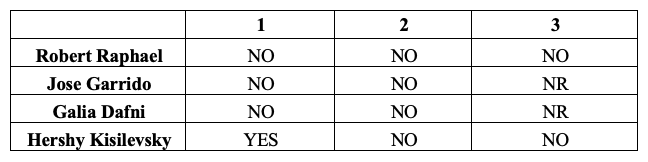
\includegraphics[scale=0.5]{images/table.png}

A pie chart was generated to facilitate the analysis of the questions.\\

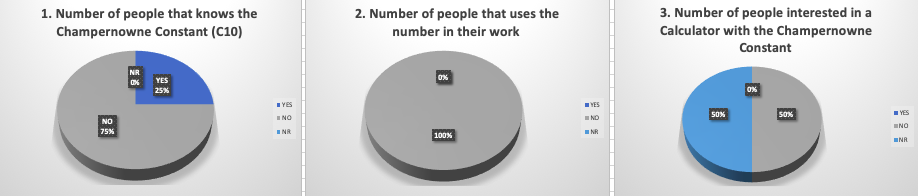
\includegraphics[scale=0.5]{images/pie.png}

The Image and Table show that only one of the persons knows about the number. This is due to the fact that he was recommended as an expert by the other potential interviewees. Even though the final interviewee knew about the number he does not uses for his work or is interested in a calculator with this number.

From this step results evident that this number is not of common knowledge even for specialist in the Math area, which makes harder to find potential users interested in a calculator.

Additionally, from the interview it is important to mention that even though the interviewee would not use a calculator for this number he established as important characteristics:

1. The multiple ways of representing the number.
2. The combination of uses between the multiple bases of the number.
3. The fact that it is a constructed number which makes it possible to identify the position of where certain patterns of number occur.
4. He would not be interested in its use for randomness.

Finally, he also said that he would prefer a calculator that can be accessed online without the need of a computer.


%----------------------------------------------------------------------------------------
\begin{thebibliography}{9}

\bibitem{bib1} 
INTRODUCTION TO INTERVIEWS.(2019).P. Kantham. Retrieve from:
\\\texttt{https://users.encs.concordia.ca/\~kamthan/courses/soen-6481/interviews\_introduction.pdf}
 
\end{thebibliography}

\end{document}
